\section{Applications of Universality}

We first introduce a couple examples, for which the connect to random matrices is not very clear. (But I promise they are related)

\begin{aexample}{Totally Asymmetric Simple Exclusion Process/ TASEP}{}
    We model a semi infinite line of electrons (or any particle). At $t=0$, all the electrons occupy the non-negative integer spaces. Particle $x_k$ is at $-k$, $k\geq 0$.

    \begin{center}
        
    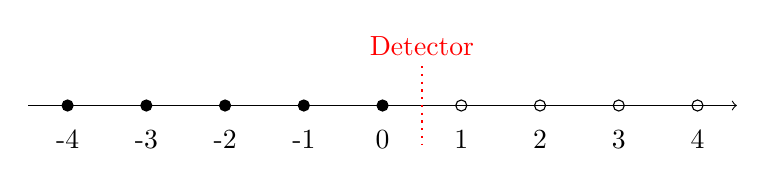
\begin{tikzpicture}[scale=1]
    % Draw the number line
    \draw[->] (-4.5,0) -- (4.5,0);
    \draw[red,thick,dotted](0.5,0.5)node[above]{Detector} -- (0.5,-0.5);
    % Draw filled dots for non-positive integers
    \foreach \x in {-4,...,0} {
        \filldraw[black] (\x,0) circle (2pt);
        \node[below] at (\x,-0.2) {\x};
    }
    
    % Draw hollow dots for positive integers
    \foreach \x in {1,...,4} {
        \draw[black] (\x,0) circle (2pt);
        \node[below] at (\x,-0.2) {\x};
    }
\end{tikzpicture}
    \end{center}

    A strong positive charge at $+\infty$ attracts the electrons independently and identically. Formally, each particle $x_k$ has an internal clock $T_k$ with distribution \[
    \mathbb{P}(T_k> s) = f(s).
    \]
    When the clock rings for $x_k$, $x_k$ will move to the right by one unit, provided that the space in front is empty (not occupied by another electron). The clock then resets to $0$ and $T_k$ is recounted again for the next time the particle moves.
    
    There is a current detector between $0$ and $1$. We want to know the following:
    
    \begin{quote}
        Given time $t>0$, what is the number of particles that passed the current detector? I.e. \[
        y_t \defeq \#\{i:x_i(t)>0\}
        \]
    \end{quote}

\end{aexample}

This was an open question for around 40 years. In the 1940's it was conjectured that \[
y_t \sim ct
\]
for a constant $c$. This was solved in 1988' by Ulm, for the case $\mathbb{P}(T_k\geq s) = e^{-s}$ which is the exponential distribution. In fact, we only understand the cases for $T_k$ is exponentially distributed, or when $T_k$ is geometrically distributed - the former being the limit of the latter. The asymptotics for general $T_k$ is widely open.

\begin{remark}
    I have heard stories about a direct competitor of my firm (one that eats into our profits) giving out this question in an interview with $T_k \sim \text{Geom}(1/2)$. Of course they made it look simple by changing the wording to `decided by a coin flip', like most quant firms. Not sure what they were looking for giving out this question to propsective intern candidates, or maybe I misunderstood and that this question was not even asked - I've never interviewed with them after all.
\end{remark}

\begin{aexample}[breakable=false]{Last Passage Percolation/ LPP}{}
    
\begin{center}
    
    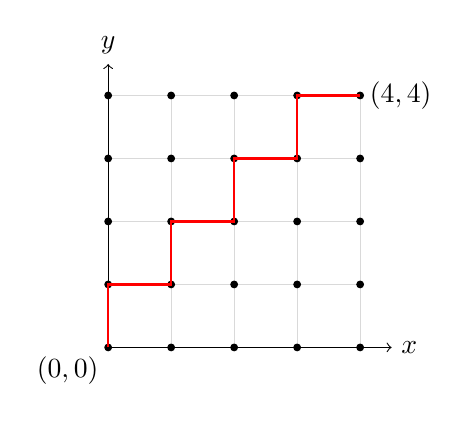
\begin{tikzpicture}[scale=0.8]
    % Draw the grid
    \foreach \x in {0,...,4} {
        \draw[gray!30] (\x,0) -- (\x,4);
    }
    \foreach \y in {0,...,4} {
        \draw[gray!30] (0,\y) -- (4,\y);
    }
    
    % Draw axes with arrows
    \draw[->] (0,0) -- (4.5,0) node[right] {$x$};
    \draw[->] (0,0) -- (0,4.5) node[above] {$y$};
    
    % Draw grid points
    \foreach \x in {0,...,4} {
        \foreach \y in {0,...,4} {
            \filldraw[black] (\x,\y) circle (1.5pt);
        }
    }
    
    % Draw a sample staircase (3,)
    \draw[red, thick] (0,0) -- (0,1) -- (1,1) -- (1,2) -- (2,2) -- (2,3) -- (3,3) -- (3,4)--(4,4);
    
    % Label start and end points
    \node[below left] at (0,0) {$(0,0)$};
    \node[right] at (4,4) {$(4,4)$};
\end{tikzpicture}

\end{center}

We now move to a 2-dimensional example. Let us cover all lattice points $v=(x\geq 0,y\geq 0)$ with an IID variable $w_v$. Fix $X,Y$ For each up-right path $\gamma$ from $(0,0) \to (X,Y)$, we let $T(\gamma)\defeq \sum_{v\in \gamma} w_v$.
What are the asymptotics of \[
L(x,y) = \max_{\gamma \text{ from } (0,0)\to (x,y)} T(\gamma)
\]
as $(x,y)\to (\infty,\infty)$, along $x=y$?

\end{aexample}
\begin{remark}
    You can read \href{https://arxiv.org/pdf/math/9903134}{Johansson} for details on this. (Later, because this spoils the fun)
\end{remark}
\begin{aexample}{Longest Increasing Subsequence}{}
    Fix N. Let $\sigma$ be a permutation of $\{1,...,N\}$ drawn uniformly in $S_N$, and $L_N$ be the longest increasing subsequence of $\sigma$. What is the asymptotic behaviour of $L_N$?  
\end{aexample}

\subsection*{TASEP is LLP}
The punchline is that these two problems are the same for exponential and geometric random variables. The first observation is that exponential and geometric random variables are memoryless i.e. \[
\mathbb{P}(T_k>n+m\ |\ T_k>m) = \mathbb{P}(T_k>n).
\]
This means we can view the internal clock in TASEP as a different clock (with the same distribution) that starts counting only if the space in front of it is empty. I will leave you to verify the details: there should be a change in the measure, but the distribution of the observable states does not change.

Now we give a mapping between $w_v$ in LLP to the states in TASEP. We imagine each particle $x_k$ lives on the line $y=k$, and they are moving to the right. The transformation is: \begin{quote}
    $w_{x,y}$ describes the time needed for particle $y$ to make the $x+1$-st step after the opportunity shows up.
\end{quote}
For instance, suppose particle $x_3$ (initially at $-3$) is now at $2$. It has taken $5$ steps already. The moment $3$ shows up empty, it takes $w_{5,3}$ time for it to move to the empty spot.


The condition for $n$ particles to pass the detector is equivalent to $x_{n-1}$ moving forward $n$ spots. So given all the internal states $w_{x,y}$, we can consider a dynamic programming approach to TASEP: Let $a_{x,y}$ describe the time needed for particle $y$ to move forward $x+1$ steps (the indexing is done to align with $w_{x,y}$). Then the base case is that \[
a_{x,y}=0
\]
if $x<0$ or $y<0$. We want particle to move $0$ steps.
The recurrance relation is
\[
a_{x,y} = \max(\underbrace{a_{x-1,y}}_{\text{particle $y$ is in previous spot}}, \underbrace{a_{x,y-1}}_{\text{next spot opens up}})+\underbrace{w_{x,y}}_{\text{particle $y$ moves}} .
\] 
This is exactly the recurrance relation for the longest path from $(0,0)$ to $(x,y)$, which is LLP!

\proposition[]{
    For geometric/exponentially distributed random variables in TASEP / LLP,

    \[
    \mathbb{P}(y_t > n)=\mathbb{P}(L(n-1,n-1)<t). 
    \]

}
\subsection*{More on the transformation}
For each state $S$ in TASEP, we can represent it as a function $f_S$ with the property \[
f_S (x) = \begin{cases*}
    f_S(x-1)+1, & \text{if }x \text{ is not occupied by a particle},\\
    f_S(x-1)-1, & \text{if }x \text{ is occupied by a particle}.
\end{cases*}
\]
This function is defined up to an arbitrary constant, so let us define function corresponding to the initial state as $|x|$.
\begin{center}\begin{tikzpicture}[scale=1]
    \draw[->] (-4.5,0) -- (4.5,0) node[right] {$x$};
    \draw[->] (0,-0.5) -- (0,4.5) node[above] {$y$};
    
    \draw[blue, thick] (-4,4) -- (0,0) -- (4,4);
    
    \foreach \x in {-4,...,0} {
        \filldraw[black] (\x,0) circle (2pt);
        \node[below] at (\x,-0.2) {\x};
    }
    
    \foreach \x in {1,...,4} {
        \draw[black] (\x,0) circle (2pt);
        \node[below] at (\x,-0.2) {\x};
    }
    
    % Label the function
    %\node[above left] at (-2,2) {$|x|$};
\end{tikzpicture}
\end{center}
When $x_0$ moves one step to the right, what happens to the graph of the state function? We would expect most of the function to be the same, except $f(0)$ and $f(1)$; those are the two places that changed `vacancy status'. Indeed, we can define the new state function as 
\begin{center}\begin{tikzpicture}[scale=1]
    \draw[->] (-4.5,0) -- (4.5,0) node[right] {$x$};
    \draw[->] (0,-0.5) -- (0,4.5) node[above] {$y$};
    
    \draw[blue, thick] (-4,4) --(-1,1)--(0,2)-- (1,1) -- (4,4);
    
    \foreach \x in {-4,...,-1,1} {
        \filldraw[black] (\x,0) circle (2pt);
        \node[below] at (\x,-0.2) {\x};
    }
    
    \foreach \x in {0,2,3,4} {
        \draw[black] (\x,0) circle (2pt);
        \node[below] at (\x,-0.2) {\x};
    }
    
    % Label the function
    %\node[above left] at (-2,2) {$|x|$};
\end{tikzpicture}
\end{center} 

This is a common way to \href{https://www.youtube.com/watch?v=QXBSxmL_Ric}{visualize TASEP}. 
We now rotate this graph 45 degrees (and rescale by $\sqrt{2}$) and superimpose it onto the LLP setup.


\begin{center}
    
    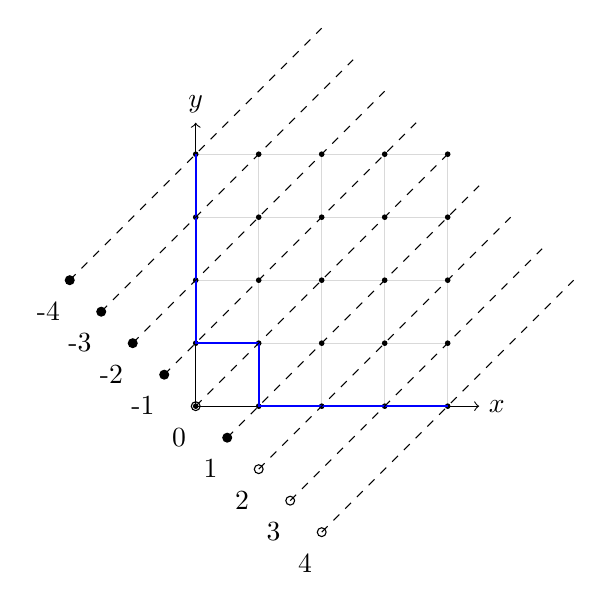
\begin{tikzpicture}[scale=0.8]
    % Draw the grid
    \foreach \x in {0,...,4} {
        \draw[gray!30] (\x,0) -- (\x,4);
    }
    \foreach \y in {0,...,4} {
        \draw[gray!30] (0,\y) -- (4,\y);
    }
    
    % Draw axes with arrows
    \draw[->] (0,0) -- (4.5,0) node[right] {$x$};
    \draw[->] (0,0) -- (0,4.5) node[above] {$y$};
    
    % Draw grid points
    \foreach \x in {0,...,4} {
        \foreach \y in {0,...,4} {
            \filldraw[black] (\x,\y) circle (1pt);
        }
    }

    \draw[blue, thick] (0,4) --(0,1)--(1,1)-- (1,0) -- (4,0);
    \foreach \x in {-4,...,4} {
        \draw[dashed,thin] (\x/2,-\x/2) -- ({4+\x/2},4-\x/2);
    }
    \foreach \x in {-4,...,-1,1} {
        \filldraw[black] (\x/2,-\x/2
) circle (2pt);
        \node[below left] at (\x/2
,-\x/2
-0.2) {\x};
    }
    
    \foreach \x in {0,2,3,4} {
        \draw[black] (\x/2
,-\x/2
) circle (2pt);
        \node[below left] at (\x/2
,-\x/2
-0.2) {\x};
    }
    
\end{tikzpicture}

\end{center}

\example[]{
    Try to convince yourself for every state, the distribution of the time it takes for the $n$-th particle to move to $m-n$ is the maximum up-right path starting from any point in the corresponding blue curve to the point $(m-1,n)$.
}


Our approach is to solving LLP is this\footnote{This is not the approach by Ulm.}: We first solve for geometric random variables then extend the result to exponential random variables as a limit of geometric.

Let $w_v \sim \text{Geom}(q)$, $0< q< 1$. That is \[
\mathbb{P}(w_v=k) = (1-q)^{k} q.
\]
Then we would have for $q=1-1/L$ as $L\to \infty$, $w_v/L \to \exp(1)$.

The value of $L(N-1,N-1)$ only depends on the $N^2$ vertices in the square $(0,0)$ -- $(N-1,N-1)$. For ease of notation, we index everything from $1$ instead of $0$ to have a matrix indexed from $1$ to $N$. We can represent this as a random matrix \[
M_{x,y} = (w_{(x,y)})
\]
with integer entries. The distribution of this matrix is given by \[
\mathbb{P}(M=A) = \prod_{i,j\leq N} \mathbb{P}(M_{i,j} = a_{i,j}) = (1-q)^{\sum a_{i,j}} q^{N^2}.
\]

This means that the frequency of each matrix only depends on the sum of the entries. Conditioned on the sum of the entries, the distribution is actually uniform over all possible matrices! So we have \begin{align*}
    \mathbb{P}(L(N-1,N-1)\leq t) =& \sum_{k=0}^{\infty} \mathbb{P}\Big(L(N-1,N-1) \ |\ \sum m_{i,j}=k\Big)\mathbb{P}\Big(\sum m_{i,j}=k\Big)\\
    =& \sum_{k=0}^{\infty} \frac{\#\overbrace{ \{L(N-1,N-1)\leq t \ |\ \sum m_{i,j}=k\}}^{\text{this is the hard part}}}{\#\underbrace{\{ \sum m_{i,j}=k\}}_{\text{not related to LPP}}} \underbrace{\mathbb{P}\Big(\sum m_{i,j}=k\Big)}_{\text{not related to LLP}}.
\end{align*}

\subsection*{LLP is Longest Increasing Subsequence}
We now translate the counting problem into longest increasing subsequence. This is a slightly different problem in that we are finding longest increasing subsequences in what is known as \textbf{generalized permutations}. 
\definition{Generalized Permutation}{
    Let $A$ be a matrix with non-negative integer entries. The \textbf{generalized permutation} associated with $A$ is defined as the two-line array \[
    \sigma_A \defeq \left(\begin{array}{ccccccccc}
        1 & 1 & ... & 1 & 1 & ... & 1&...&N\\
        \undermat{a_{1,1} \text{ times}}{1 & 1 & ... & 1} & \undermat{a_{1,2} \text{ times}}{2 & ... & 2} &...&N\\
    \end{array}\right).
    \] 
    \\
    
    
}
\begin{aexample}{}{}
    Let $A$ be a permutation matrix. Then $\sigma_A$ is in the form \[
    \begin{bmatrix}
        1 & 2 &... & N\\
        \sigma(1) & \sigma(2) & ... &\sigma(N)
    \end{bmatrix}
    \]
    which is the standard two-line representation of a permutation.
\end{aexample}

\proposition{
    Given the matrix $M$, $L(N-1,N-1)$ is the length of the longest increasing subsequence of $\sigma_{M^T}$.
}
\begin{proof}[Idea of proof]
    For every path in $\gamma$ from $(0,0)$ to $(N-1,N-1)$, associate to an increasing subseqeunce in $\sigma_{M^T}$ (Hint: just take all the indices the path visited), and the length of the subsequence is the sum of weights. For every increasing subseqeunce, we can extend it to a longer subsequence (for each index $i,j$, we can take all of the columns or none of the columns) and it corresponds to a path with sum of weights equal to the length of the extended subseqeunce.
\end{proof}